%Header for the instruction files


%%%%%%%%%%%%%%%%%%%%%%%%%%%%%%%%%%%%%%%%%%%% PACKAGES %%%%%%%%%%%%%%%%%%%%%%%%%%%%%%%%%%%%%%%%%%%%%%%%%%%%%%%%%

%euopean version of article, because paper format is A4
\documentclass{scrartcl}

\usepackage[a4paper, left=5mm, right=10cm, top=1cm, marginparwidth=9cm]{geometry}

%UTF-8, because want decent encoding
\usepackage[utf8]{inputenc}

%\usepackage[ngerman]{babel}

%for ae ue oe
%\usepackage{ae}
\usepackage[T1]{fontenc}

%better monospaced font
\usepackage[scaled=0.8]{beramono}

%to have math symbols available
\usepackage{amsmath,amssymb,euscript}

%pretty enumerations
\usepackage{enumerate}

\usepackage{physics}

\usepackage{mathtools}

%pictures 
\usepackage{graphicx}
%\DeclareGraphicsRule{.tif}{png}{.png}{`convert #1 `dirname #1`/`basename #1 .tif`.png}

%listings are a nice way to display source code
\usepackage{listings, color}
\usepackage[table]{xcolor}

%define another version of green in addition to the 16 tex colors
\definecolor{mygreen}{rgb}{0.133,0.545,0.133}

%for weblinks
\usepackage[hidelinks]{hyperref}

\usepackage{mdframed}

\usepackage{tocloft}

\usepackage{marginnote}

\usepackage{tabularx}

\usepackage{ textcomp }

%%%%%%%%%%%%%%%%%%%%%%%%%%%%%%%%%%%%%%%%%%%% COMMANDS AND SETTINGS %%%%%%%%%%%%%%%%%%%%%%%%%%%%%%%%%%%%%%%%%%%%


%noindent, because text passages are very short to begin with
\setlength\parindent{0pt}

%instead the distance between lines is a bit bigger, if a paragraph ends
%this is a default value, it is sometimes changed locally, for example whenever itemize is used
%\setlength{\parskip}{1.0cm plus4mm minus3mm}

%use these commands when you want to create a list of points using itemize
%the distance between paragraphs defined above makes lists look very bad, use /nogap before creating a list and \gap after to restore settings
\newcommand{\nogap}{}%\setlength{\parskip}{0.0cm}}
\newcommand{\gap}{}%\setlength{\parskip}{1.0cm plus4mm minus3mm}}


%command that configures the code listings to be in a box with line numbers to the left
%it also makes sure that there is space between the last paragraph and the source code, so make sure you use this command before every 
%listing of a complete program
\newcommand{\numbersleft}{ 
\setlength{\parskip}{0cm}
{\scriptsize \mbox{}} \\ 
\setlength{\parskip}{1.0cm plus4mm minus3mm}
\lstset{ %
  language=C++, % choose the language of the code
  basicstyle=\footnotesize\ttfamily, % the size of the fonts that are used for the code
  numbers=left, % where to put the line-numbers
  numberstyle=\footnotesize\ttfamily\color[rgb]{0.6,0.6,0.6}, % the size of the fonts that are used for the line-numbers
  stepnumber=1, % the step between two line-numbers. If it's 1 each line
  xleftmargin=1mm,
  xrightmargin=1mm,
  % will be numbered
  numbersep=10pt, % how far the line-numbers are from the code
  backgroundcolor=\color{white}, % choose the background color. You must add \usepackage{color}
  showspaces=false, % show spaces adding particular underscores
  showstringspaces=false, % underline spaces within strings
  showtabs=false, % show tabs within strings adding particular underscores
  %frame=l, % adds a frame around the code
  frame=single,
  tabsize=4, % sets default tabsize to 2 spaces
  breaklines=true, % sets automatic line breaking
  breakatwhitespace=false, % sets if automatic breaks should only happen at whitespace
  % also try caption instead of title
  escapeinside={\%*}{*)}, % if you want to add a comment within your code
  morekeywords={*,...}, % if you want to add more keywords to the set
  keywordstyle=\color[rgb]{0,0,1},
  commentstyle=\color[rgb]{0.133,0.545,0.133}\textit,
  stringstyle=\color[rgb]{0.627,0.126,0.941},
}}

%command that configures the code listings to be without a box and without line numbers to the left
%it also makes sure that there is space between the last paragraph and the source code, so make sure you use this command before every listing which
%is just a code snippet
\newcommand{\nonumbers}{
\setlength{\parskip}{0cm}
{\scriptsize \mbox{}} \\ 
\setlength{\parskip}{1.0cm plus4mm minus3mm}
\lstset{ %
  language=C++, % choose the language of the code
  basicstyle=\footnotesize\ttfamily, % the size of the fonts that are used for the code
  numbers=none, % where to put the line-numbers
  numberstyle=\footnotesize\ttfamily\color[rgb]{0.6,0.6,0.6}, % the size of the fonts that are used for the line-numbers
  stepnumber=1, % the step between two line-numbers. If it's 1 each line
  xleftmargin=4mm,
  % will be numbered
  numbersep=5pt, % how far the line-numbers are from the code
  backgroundcolor=\color{white}, % choose the background color. You must add \usepackage{color}
  showspaces=false, % show spaces adding particular underscores
  showstringspaces=false, % underline spaces within strings
  showtabs=false, % show tabs within strings adding particular underscores
  frame=none, % adds a frame around the code
%  frame=single,
  tabsize=4, % sets default tabsize to 2 spaces
  breaklines=true, % sets automatic line breaking
  breakatwhitespace=false, % sets if automatic breaks should only happen at whitespace
  % also try caption instead of title
  escapeinside={\%*}{*)}, % if you want to add a comment within your code
  morekeywords={*,...}, % if you want to add more keywords to the set
  keywordstyle=\color[rgb]{0,0,1},
  commentstyle=\color[rgb]{0.133,0.545,0.133}\textit,
  stringstyle=\color[rgb]{0.627,0.126,0.941},
}}


%default configuration for lstset, so lstinline fragments are displayed correctly before the first lstlisting appears
\lstset{ %
  language=C++, % choose the language of the code
  basicstyle=\footnotesize\ttfamily, % the size of the fonts that are used for the code
  numbers=none, % where to put the line-numbers
  numberstyle=\footnotesize\ttfamily\color[rgb]{0.6,0.6,0.6}, % the size of the fonts that are used for the line-numbers
  stepnumber=1, % the step between two line-numbers. If it's 1 each line
  xleftmargin=4mm,
  % will be numbered
  numbersep=5pt, % how far the line-numbers are from the code
  backgroundcolor=\color{white}, % choose the background color. You must add \usepackage{color}
  showspaces=false, % show spaces adding particular underscores
  showstringspaces=false, % underline spaces within strings
  showtabs=false, % show tabs within strings adding particular underscores
  frame=none, % adds a frame around the code
%  frame=single,
  tabsize=4, % sets default tabsize to 2 spaces
  breaklines=true, % sets automatic line breaking
  breakatwhitespace=false, % sets if automatic breaks should only happen at whitespace
  % also try caption instead of title
  escapeinside={\%*}{*)}, % if you want to add a comment within your code
  morekeywords={*,...}, % if you want to add more keywords to the set
  keywordstyle=\color[rgb]{0,0,1},
  commentstyle=\color[rgb]{0.133,0.545,0.133}\textit,
  stringstyle=\color[rgb]{0.627,0.126,0.941},
}


%newcommands for exercises and solutions
\newcounter{excounter} \setcounter{excounter}{0}
\newcounter{partexcounter} \setcounter{partexcounter}{0}
\newcommand{\exercise}[1]{\stepcounter{excounter}\setcounter{partexcounter}{0}\vspace*{10px} \noindent \textbf{\textsf{Exercise \arabic{excounter})\quad #1}}\quad \\}
\newcommand{\partexercise}{\stepcounter{partexcounter}\noindent \textbf{\textsf{(\alph{partexcounter})}}\quad}

\newcounter{partsolcounter} \setcounter{partsolcounter}{0}
\newcommand{\solution}[1]{\vspace*{10px} \noindent \textbf{\textsf{Solution \arabic{excounter})}} \quad \textit{#1}\\}
\newcommand{\partsolution}{\stepcounter{partsolcounter} \noindent \textbf{\textsf{(\alph{partsolcounter})}}\\}


%reminder to answer students' questions
\newcommand{\quest}{\begin{center}
                    \Large{\textit{Questions?}}
                    \end{center}
}


% header and footer definitions if someone wants to introduce headers and footers to the sheets
%
%\usepackage{fancyhdr}
%\pagestyle{fancy}
%\fancyhf{}
%
% upper right
%\fancyhead[R]{\textsf{Exercise something}}
%
% upper left 
%\fancyhead[L]{whatever}
%
% upper middle
%\fancyhead[C]{\textbf{Exercise Class 1}}
%
% lower middle
%\fancyfoot[C]{\textsf{Seite \thepage}}
%
% lower left 
%\fancyfoot[L]{\textsf{\today}}
%
% lower right
%\fancyfoot[R]{\textsf{blabla}}

\newcommand{\strong}[1]{\textbf{#1}}
\newcommand{\slide}[1]{\textbf{slide #1}}
\newcommand{\critical}[1]{\textcolor{red}{\textbf{#1}}}
\newcommand{\TODO}[1]{\textbf{TODO: #1}}
\newcommand{\Expert}{[code]expert}
\newcommand{\Codeboard}{Codeboard}
\newcommand{\ExerciseClass}[1]{%
\begin{center}
	\LARGE{\textbf{\textsf{Exercise Class \the\numexpr #1 \relax}}}
\end{center}}

\newcommand{\blackboard}{blackboard}
\newcommand{\slides}{slides}
\newcommand{\ide}{programming environment}
\newcommand{\PreparationSection}[1]{\section{\textcolor{red}{Preparation: #1}}}
\newcommand{\ImportantSection}[2]{\section{\textcolor{red}{#1} (#2 min.)}}
\newcommand{\MandatorySection}[2]{\section{\textcolor{red}{#1} (#2 min.)}}
\newcommand{\OptionalSection}[2]{\section{#1 (#2 min.)}}
\newcommand{\AdditionalMaterialSection}[2]{%
\marginnote{%
    The additional material sections provide some additional classroom
    activities which you can use in case you decide that the provided
    lesson plan does not work for you.
}[1cm]
\section{Additional Material: #1 (#2 min.)}}
\newcommand{\SubSectionInformational}[1]{\subsection{#1}}
\newcommand{\SubSection}[1]{\subsection{#1}}
\newcommand{\SubSectionWith}[2]{\subsection{#1 (#2)}}
\newcommand{\SubSectionWithTime}[3]{\subsection{#1 (#2 min., #3)}}
\newcommand{\SubSectionExplanation}[2]{\subsection{Explanation (#1 min., #2)}}
\newcommand{\SubSectionExplanationOptional}[2]{\subsection{(Optional) Explanation (#1 min., #2)}}
\newcommand{\SubSectionExercise}[2]{\subsection{Exercise: #1 (#2 min.)}}
\newcommand{\SubSectionExerciseTask}[2]{\subsubsection{Task (#1 min., #2)}}
\newcommand{\SubSectionExerciseThink}[1]{\subsubsection{Reading Task and Individual Thinking (#1 min.)}}
\newcommand{\SubSectionExercisePair}[1]{\subsubsection{Pair Programming (#1 min., \ide{})}}
\newcommand{\SubSectionExerciseIndividual}[1]{\subsubsection{Individual Programming (#1 min., \ide{})}}
\newcommand{\SubSectionExercisePairDiscuss}[1]{\subsubsection{Pair Discussion (#1 min.)}}
\newcommand{\SubSectionExercisePairDiscussShare}[1]{\subsubsection{Pair Programming, Discussion and Share Solution (#1 min.)}}
\newcommand{\SubSectionExerciseShare}[1]{\subsubsection{Share Solution (#1 min., \ide{})}}
\newcommand{\SubSectionExerciseShareSolution}[2]{\subsubsection{Share Solution (#1 min., #2)}}
\newcommand{\SubSectionExerciseSolution}[2]{\subsubsection{Solution (#1 min., #2)}}

\newcommand{\listofpreparationtasks}{Prepare Before the Class}
\newlistof{preparationtask}{lex}{\listofpreparationtasks}

\mdfdefinestyle{Preparation}{%
frametitle={Preparation},
backgroundcolor=black!10,
bottomline=false,
topline=false,
rightline=false,
leftline=false
}
\newenvironment{Preparation}{%
\newcommand{\PreparationBeforeClass}[1]{%
\addcontentsline{lex}{preparationtask}{$\square$ ##1}%
$\square$ ##1\\}
\newcommand{\PreparationInClass}[1]{$\square$ ##1\\}
\begin{mdframed}[style=Preparation]%
}{%
\end{mdframed}%
}

\mdfdefinestyle{Question}{%
frametitle={Question},
}
\newenvironment{Question}{%
\newenvironment{Answer}{\hfill\\[1em]\strong{Possible Answer}\\}{}
\newenvironment{OnlyAnswer}{\hfill\\[1em]\strong{Answer}\\}{}
\begin{mdframed}[style=Question]%
}{%
\end{mdframed}%
}


\mdfdefinestyle{Explanation}{%
backgroundcolor=black!5,
}
\newenvironment{Explanation}{%
\begin{mdframed}[style=Explanation]%
}{%
\end{mdframed}%
}

\newenvironment{Theory}{%
\section*{Theory}

The theory points of this exercise session are:
\begin{enumerate}}{\end{enumerate}}

\newenvironment{SeenInClass}{%
\section*{Seen in class}
During the last class, students have seen:
}



% Some commands copied from the exam.
\newcommand{\rmin}{\mathrm{min}}
\newcommand{\rmax}{\mathrm{max}}
\newcommand{\boxx}[3]{\begin{minipage}[c][#3]{#2}#1~ \end{minipage}}



\begin{document}

\ExerciseClass{1}

\begin{Theory}
\item Sobolev spaces
\item Linear Variational Problems
\item Equilibrium Models: Boundary Value Problems
\item Diffusion Models: Stationary Heat Conduction
\item Boundary Conditions
\item Second-Order Elliptic Variational Problems
\item Essential and Natural Boundary Conditions
\end{Theory}

\section*{Exercises}

The exercises reviewed in this exercise class are:
\begin{itemize}
    \item Problem 1-1: Quadratic Functionals, only sub-problems a) b) d) g) (50 min)
    \item Problem 1-2: Linear functionals on Sobolev spaces, a) b), e) f) g) only (90 min)
    \item Problem 1-5: A second-order elliptic transmission problem in 1D (75 min)
    \item Problem 1-6: Heat conduction with non-local boundary conditions (55 min)
    \item Problem 1-7: A second-order boundary value problem for vector fields (110 min)
\end{itemize}

% \listofpreparationtask


\tableofcontents

\newpage

\OptionalSection{A journey: From Quadratic Minimization Problems on Sobolev Spaces to PDEs through LVPs}{55}

\SubSectionWith{Introduction}{5min} 

Show on the blackboard your favorite quadratic minimization problem and a PDE. Note that we introduce ambiguity on purpose in the formulation for later use (no config space + no BDC). Note also that $\sigma$ doesn't depend on x for simplification.
\begin{equation}
    J_s(u) = \int_a^b \frac{1}{2}\sigma (\frac{du}{dx}(x))^2 - f(x)u(x) dx
\end{equation}
\begin{equation}
    u = \text{argmin}_v \ J_s(v)
\end{equation}
\begin{equation}
    -\sigma  u'' = f
\end{equation}

Start by stating what are the goals of this session:
\begin{enumerate}
    \item Give them an overview of the notions of quadratic minimization problems, LVPs and PDEs
    \item Give them the tools to convert from one formulation of the problem to another
    \item Have an intuitive understanding of Sobolev Spaces and their norms
    \item Understand boundary conditions and which makes sense for a given PDE
\end{enumerate}

\SubSectionWith{Quadratic Minimization Problems}{5min}

\begin{enumerate}
    \item 
Take your favorite energy potential, e.g. the 1d elastic string under vertical loading. Show an interactive example of it, e.g. the interactive elastic rod example from \url{https://gitlab.ethz.ch/yueliyue/pbs22/-/tree/master/2_fem}. 
\begin{equation}
    J_s(u) = \int_a^b \frac{1}{2}\sigma (\frac{du}{dx}(x))^2 - f(x)u(x) dx
\end{equation}

You could also optionally derive it. For this particular example, from Hook's law on the strain energy of an elastic rod with nodes $x_i$. 
\begin{equation}
    \epsilon = \frac{\Delta l_i}{L_i} = \frac{u(x_{i+1}) - u(x_i)}{x_{i+1} - x_i} \xrightarrow{\Delta x \rightarrow 0} \frac{du}{dx}(x)
\end{equation}
\begin{equation}
    E_{elastic} = \frac{1}{2}\sigma\epsilon^2
\end{equation}

With $u(x) = x - x'$ being the displacement field from original to deformed state.

\item
Introduce Equilibrium principle: a system tends to its minimum energy configuration. Ask to the students what is missing in the minimization equation that is on the board:
\begin{equation}
    u = \text{argmin}_v \ J_s(v)
\end{equation}

Configuration space is missing, introduce configuration space: space (=set) of functions that we want to search, depends on the problem we are solving. E.g., for 1d string we want it to be continuous:
\begin{equation}
    V = \{u \in C^0([a, b]), u(a) = u_0, u(b) = u_1\}
\end{equation}

Ask the students what is the problem with the presented configuration space and potential: we are asking for the derivative of u but our configuration space includes non-differentiable functions!
Thus we need to constrain our space more (draw example of $C^1_{pw}$ function).

\begin{equation}
    V = \{u \in C^1_{pw}([a,b]), u(a) = u_0, u(b) = u_1\}
\end{equation}
\end{enumerate}

\SubSectionWith{Sobolev Spaces}{10min}
Note: when we say that X is integrable, it means that the integral of X is smaller than $\infty$

Motivation for Sobolev Spaces:
\begin{enumerate}
    \item Introduce potential$$J(u) = \int_0^1 \frac{1}{2}u(x)^2 - u(x) dx$$ with space for the problem $C^0_0([0,1])$.
    \item Rewrite it as $$J(u) = \frac{1}{2}\int_0^1 (u(x) - 1)^2 - 1 dx$$.
    \item Draw on the blackboard the sequence of functions that minimize J(u) starting by a parabola, from the intuition that we this is like a penalty for when $u(x)$ != 1, and u(x) is continuous, then every point should tend to 1. Our trial space of u is too small!
    \item Introduce $L^2(\Omega)$, the space of square integrable functions, largest space in which this problem still make sense
    $$\int_\Omega |v(x)|^2 dx < \infty $$ with associated norm
    $$(\int_\Omega |v(x)|^2 dx)^\frac{1}{2} $$,
    \item In this space (at the end we really only care about the norm), there exist a solution to the problem, but the boundary conditions are not compatible with this norm. We'll see later more about compatible BCs.
\end{enumerate}
End of motivation.

Going back to our original potential:
\begin{enumerate}
    \item For our above problem, we saw that we needed more than just continuity as we're using derivatives in the expression. Introduce $H^1_0(\Omega)$, space of integrable functions with square integrable gradient with values 0 on the boundaries:
    $$\int_\Omega ||grad \ v(x)||^2 dx < \infty $$ 
    with norm
    $$|v|_{H^1_0(\Omega)} = (\int_\Omega ||grad \ v(x)||^2 dx)^\frac{1}{2}$$
    \item Note that here we are imposing BCs but we saw before in $L^2$ that they didn't make sense. Going back to the example from before, we see that the function has a very steep gradient at the borders: the minimizer won't be the one leaving out the BCs as it's gradient would be infinitely big!
    \item Finally, quickly introduce $H^1(\Omega)$, with norm
    $$||v||_{H^1(\Omega)} = |v|_{H^1(\Omega)} + ||v||_{L^2(\Omega)}$$
    \item Introduce the meaning of super/subscripts in Sobolev spaces: superscript := derivative, subscripts := BCs.
    \item Finally reassure the students that Sobolev spaces are simply a useful tool for energy minimization problems, that we're primarly interested in their norms and that one can see as a replacement of
    $$L^2(\Omega) \rightarrow C^0_{pw}(\Omega), \quad H^1_0{\Omega} \rightarrow C^1_{pw,0}$$
\end{enumerate}

Correspondance between piecewiese continuity and sobolev spaces; norms of sobolev spaces


\SubSectionWith{Linear Variational Problems}{10min}
Introduce this section by explaining that this is the formulation that we prefer for solving quadratic minimization problems, as in finite dimensions solving a linear variational problem reduces to solving a LSE, which we learnt in NumCSE how to solve efficiently. 

Introduce the definition of a finite quadratic functional on $\mathbb{R}^n$: $ J(\eta) = \frac{1}{2}\eta^TA\eta - \beta^T\eta + c$. Remember that we want to minimize this functional, thus we want to set its gradient to 0. Knowing that its gradient is given by (you don't have to derive it, just give the 1D intuition) $\textbf{grad} \ J = A\eta - \beta =^! 0 $, we have that $A\eta = \beta$ which is a LSE that we know how to solve from NumCSE. Finite dimensional quadratic functionals are thus a nice form for our initial quadratic minimization problem, but how do we arrive at them from our initial potential?


\begin{enumerate}
\item Introduce def. of linear form: $l : V_0 \to \mathbb{R}$, $l(\alpha u + \beta v) = \alpha l(u) + \beta l(v)$

\item Introduce def. of bilinear forms: $a(\alpha u_1 + u_2, \beta v_1 + v_2 ) = \alpha \beta a(u_1, v_1) + \alpha a(u_1, v_2) + \beta a(u_2, v_1) + a(u_2, v_2)$. Five them the trick that the coefficients of $a(a+b, c+d)$ behave like the one of a multiplication $(a+b)*(c+d)$.
\item Introduce p.d $a(v,v) > 0 \text{ and } a(0, 0) = 0$ and introduce s.p.d $a(v,v) \geq 0$. 
\item Introduce quadratic functional $$J(u) := \frac{1}{2} a(u,u) - l(u) + c  \quad u \in V$$

\item Recast $J_s(v)$ in term of a quadratic functional (match definition of quadratic functional with existing potential formulation):
\begin{equation}
    J_s(u) = \frac{1}{2} a(u,u) - l(u)
\end{equation}
\begin{equation}
    \frac{1}{2} a(u,u) = \frac{1}{2}\sigma \int_a^b  \frac{du}{dx}(x)\frac{du}{dx}(x) dx \quad
    l(u) = \int_a^b f(x)u(x) dx
\end{equation}

\item Remember how previously we took the gradient of our finite dimensional quadratic functional to find the solution of our minimization problem? As we are in infinite dimensions, we have to define an auxiliary function that help us understanding how the functional is affected by local changes in any "direction". u is the searched solution for our minimization problem, v an arbitrary "direction" in which we want to analyze the change of value of the functional, $\phi_v : \mathbb{R} \rightarrow \mathbb{R}$:

\begin{equation}
\begin{aligned}
    \phi_v(t) &= J(u + tv) \\ &= \frac{1}{2}t^2a(v,v) + ta(u,v) + \frac{1}{2}a(u,u) - tl(v) - l(u)
\end{aligned}
\end{equation}

As $\phi_v$ is an upward parabola, it's derivative is 0 at $t=0$: $$\phi'(0) = a(u,v) - l(v) = 0$$ for any arbitrary "direction" v, and thus this gives rise to what we call a linear variational problem: $$a(u,v) = l(v), \quad \forall v \in V_0$$
\end{enumerate}

This is still an infinite dimensional problem that we can't solve directly, but tell the students that we'll see next week the best way to reduce a quadratic functional on an infinite dimensional function space to a finite one to then be able to solve it as a LSE (=the essence of this course), keyword: Galerkin Projection. (Hype!)



\SubSectionWith{Example solving}{5min}

Solve subexercise 1.1.b as an additional example on how to identify quadratic functionals from energy potentials. Show them how you can find a counter example: you want a second derivative that is not zero and a first derivative that is negative.



\SubSectionWith{Boundary Value Problems for PDEs}{10min}
It's time to end our journey and formulate the problem in yet another way: the language of PDEs. PDEs are the language that you mostly see problems written as, arising naturally from a continuum approach (thinking about the infinitesimally small) to diverse physical problems. They are used in many fields of applications, and understanding them and knowing how to solve them numerically is a core component of this course. 
PDEs arise naturally from variational problems:

\begin{figure}[h]
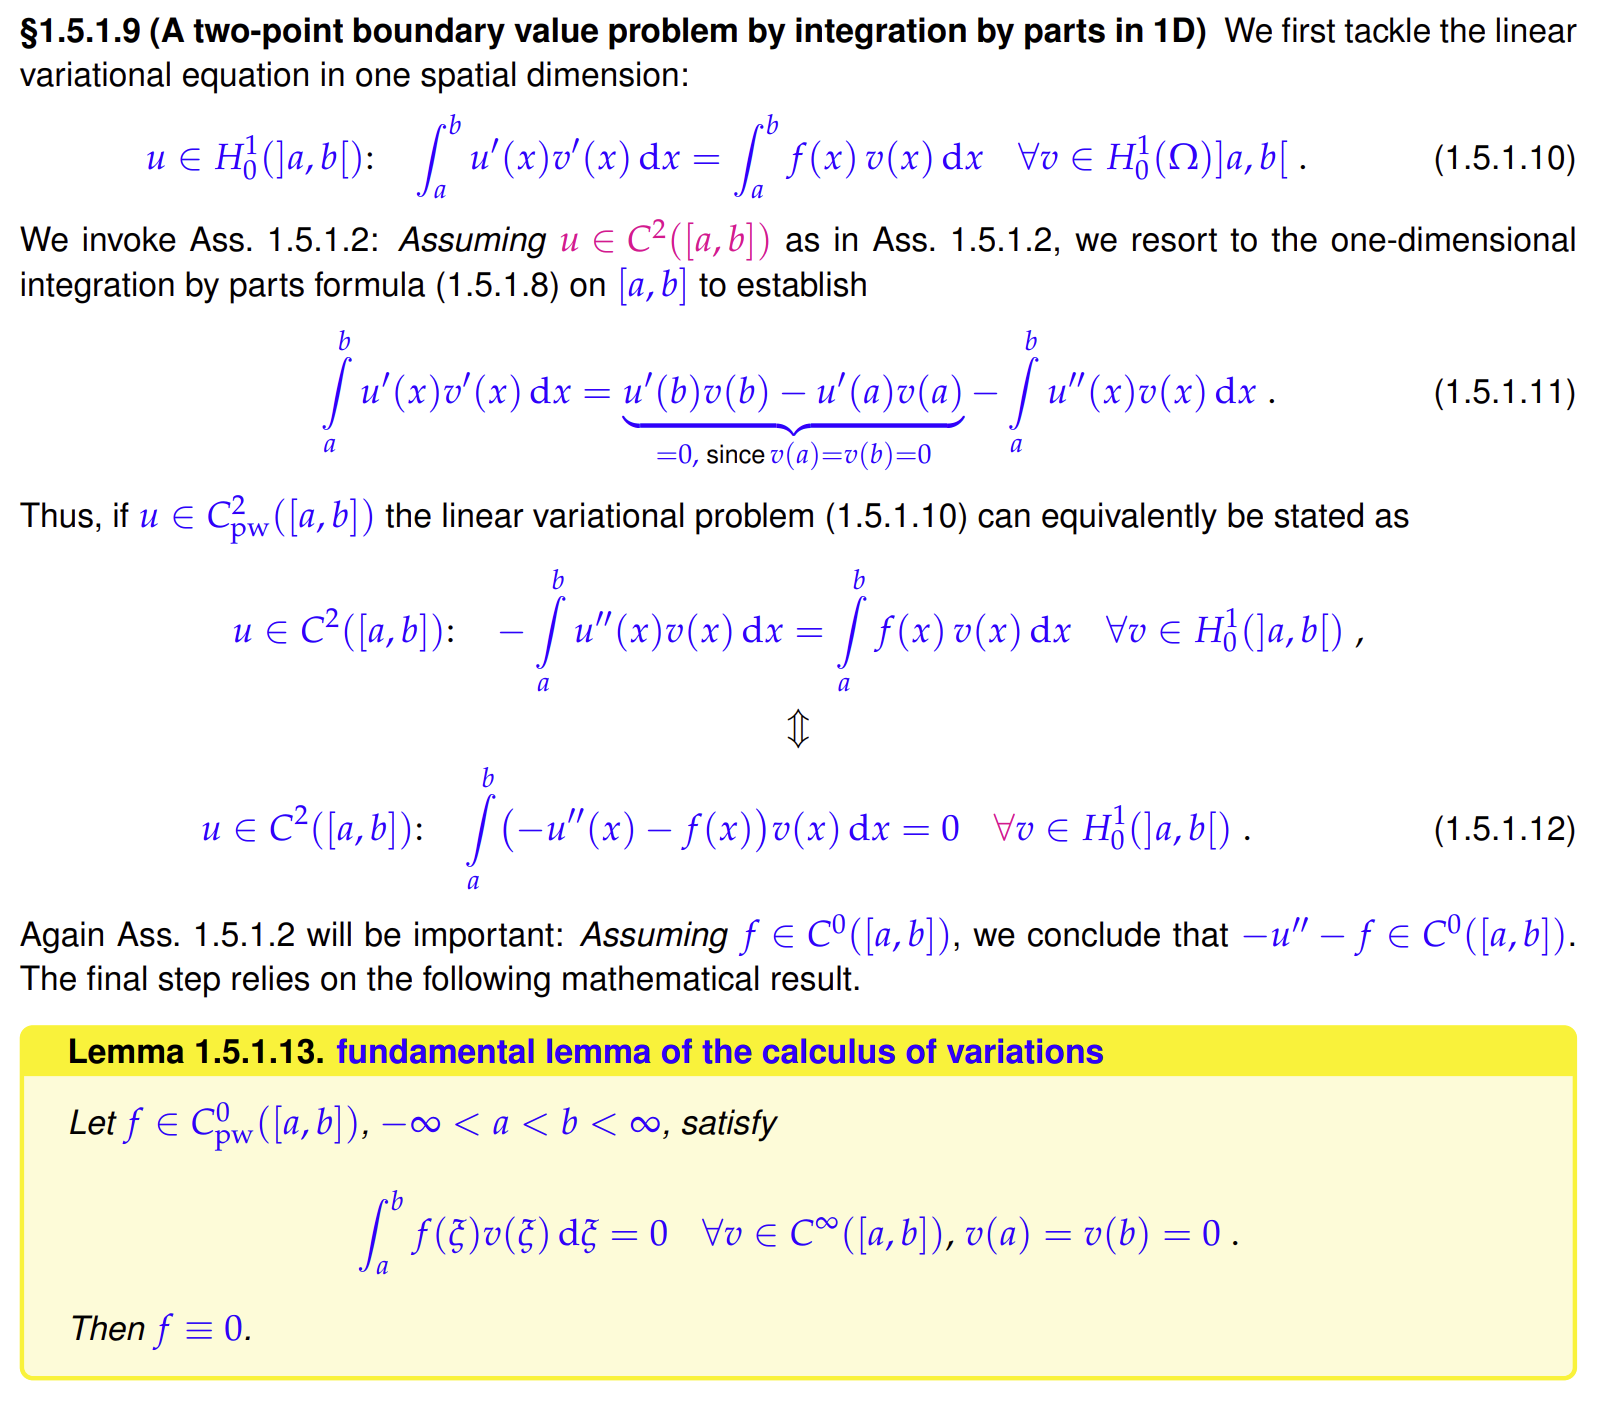
\includegraphics[]{week02/lvp_to_pde.png}
\end{figure}

At the end, we get:
\begin{equation}
    -u''(x) = f(x) \quad \forall x \in ]a, b[, \quad u(a) = 0, u(b) = 0
\end{equation}

Note that we call PDEs "Strong" formulations as we need extra smoothness requirements to express the problem.



\SubSectionWith{Boundary Conditions}{10min}
TODO
Introduce Dirichlet + Neumann BC. Speak about Compatibility condition. Explain why essential vs natural respectively.



\OptionalSection{Solving Exercises}{35min}

\SubSectionWith{From Weak to Strong formulation in higher dimensions}{10min}

Start with recap:

\textbf{General product rule} \newline
for all $\mathbf{j} \in (C^1(\Bar{\Omega}))^d, v \in C^1(\Bar{\Omega})$ holds $$\text{div} (\mathbf{j}v) = v\, \text{div}\, \mathbf{j} + \mathbf{j \cdot grad} v \quad\text{in}\, \Omega$$

\textbf{Gauss` Theorem} \newline
let $\mathbf{n} : \partial \Omega\rightarrow \mathbb{R}^d$ denote the exterior unit normal vector field on $\partial\Omega$ and $dS$ denote integration over a surface, we have $$\int_\Omega \text{div}\, \mathbf{j(x)dx} = \int_{\partial\Omega} \mathbf{j(x)\cdot n(x)}dS(x)\quad \forall \mathbf{j} \in (C^1_{pw}(\Bar{\Omega}))^d$$

\textbf{Green`s first formula} \newline
for all vector fields $\mathbf{j} \in (C^1_{pw}(\Bar{\Omega}))^d$ and functions $v\in C^1_{pw}(\Bar{\Omega})$ holds $$\int_\Omega \mathbf{j \cdot grad}v \mathbf{dx} = - \int_\Omega \text{div}\,\mathbf{j}v\mathbf{dx} + \int_{\partial\Omega} \mathbf{j \cdot n} v\, dS$$

Solve exercise 1.6 a,b,d:


\begin{enumerate}
    \item Identify bilinear form and linear form
    \item Argue why bilinear form is P.D.
    \item Derive PDE from LVP
\end{enumerate}

\begin{figure}
\centering
    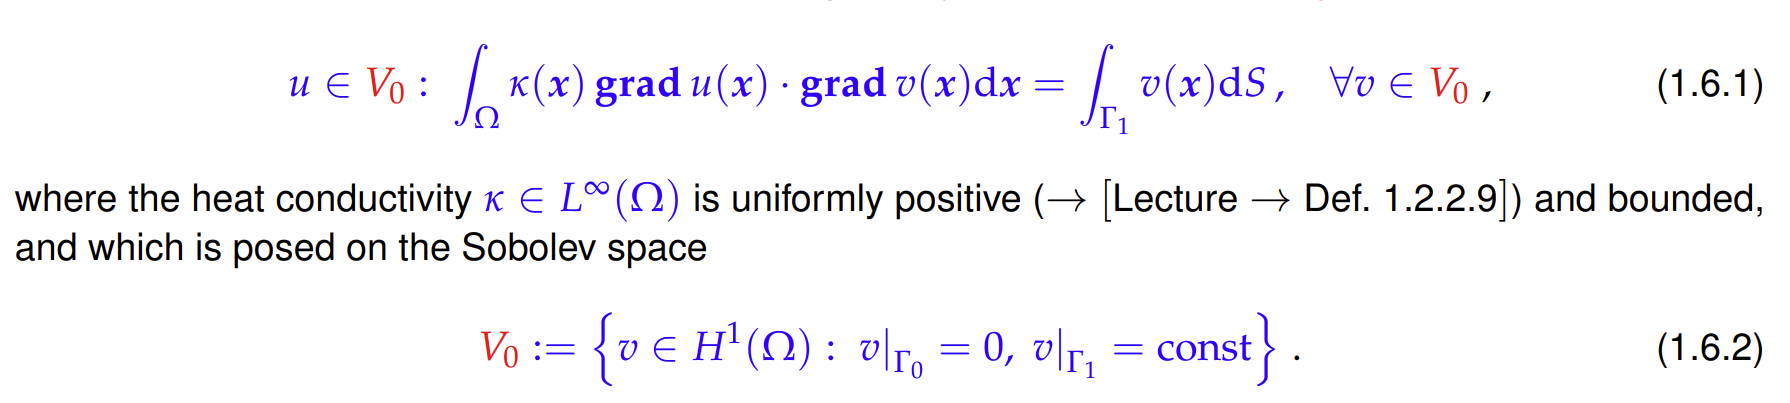
\includegraphics{week02/ex1_6_1.png}
    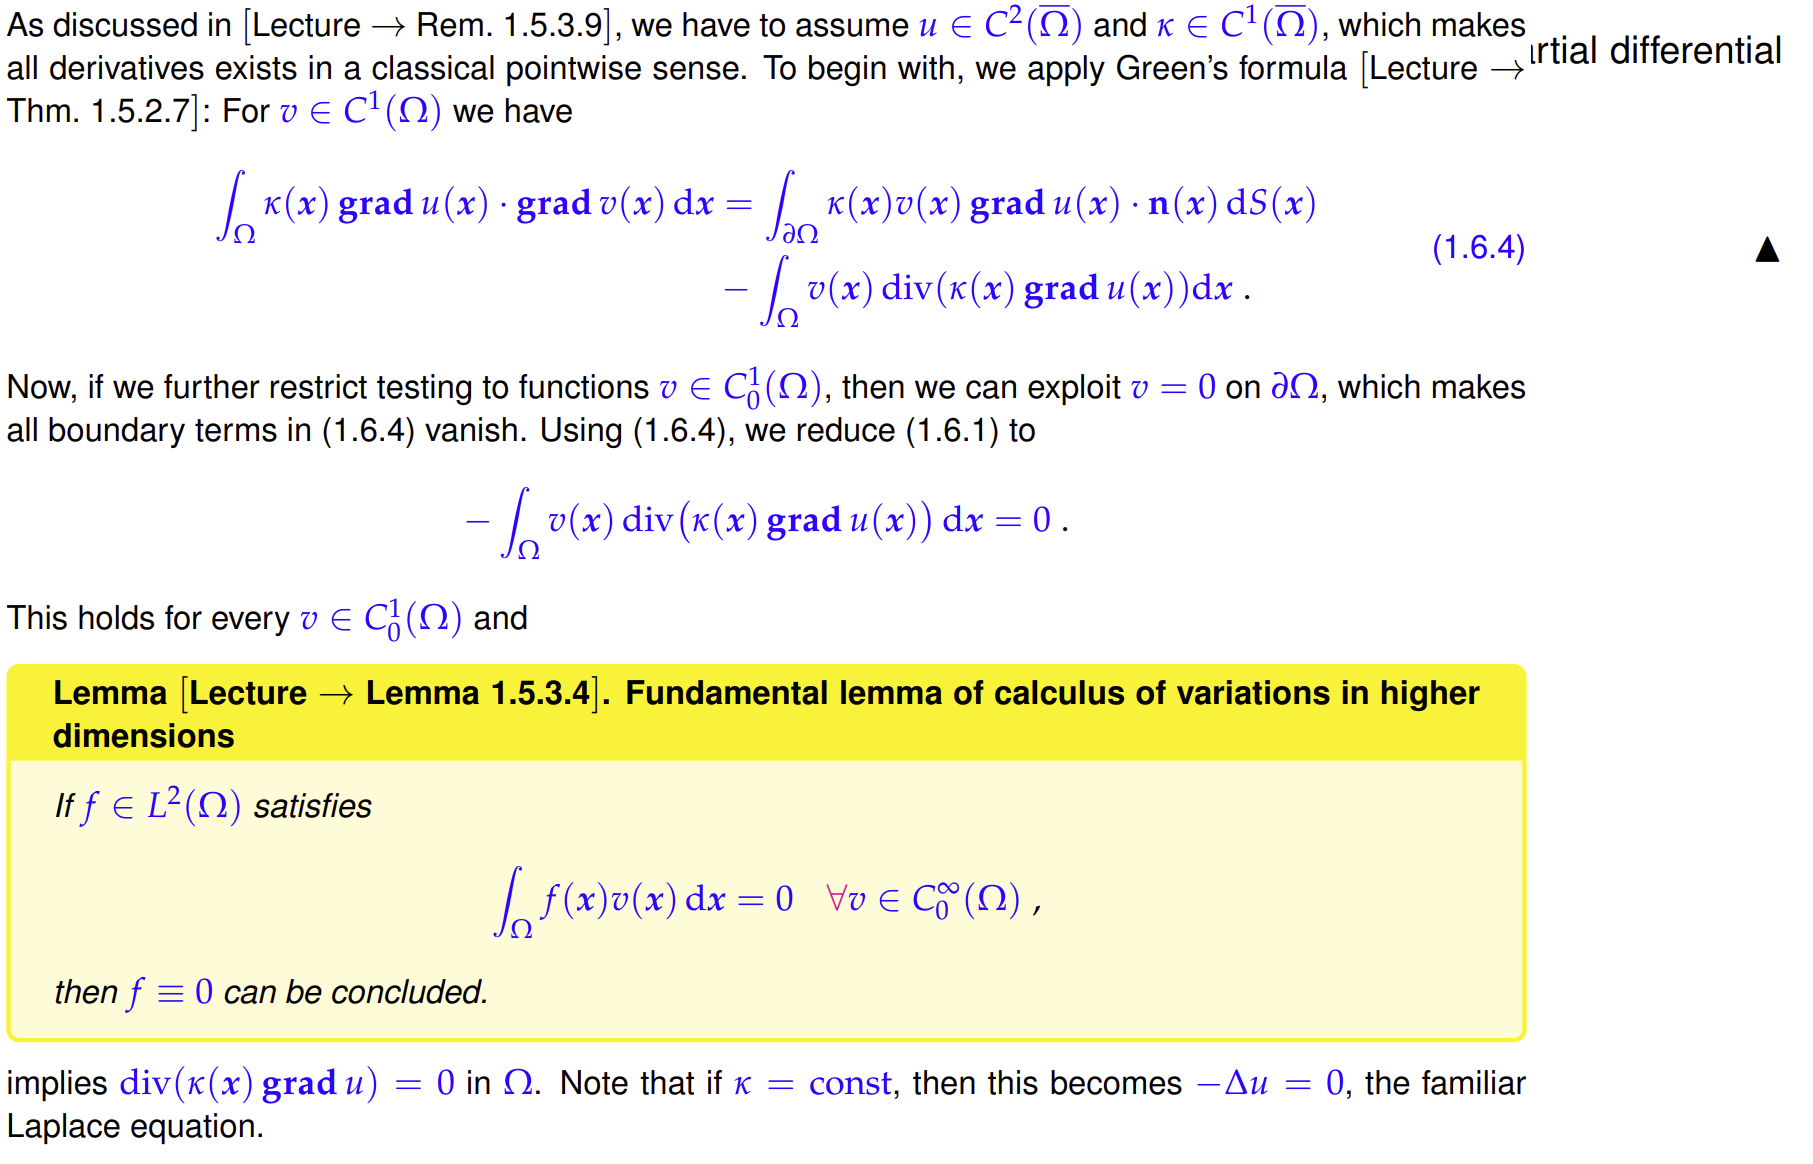
\includegraphics{week02/ex1_6_sol.png}
\end{figure}

\SubSectionWith{From Strong to Weak formulation}{10min}

TODO: FIND EXERCISE FROM EXAM

\begin{figure}
\centering
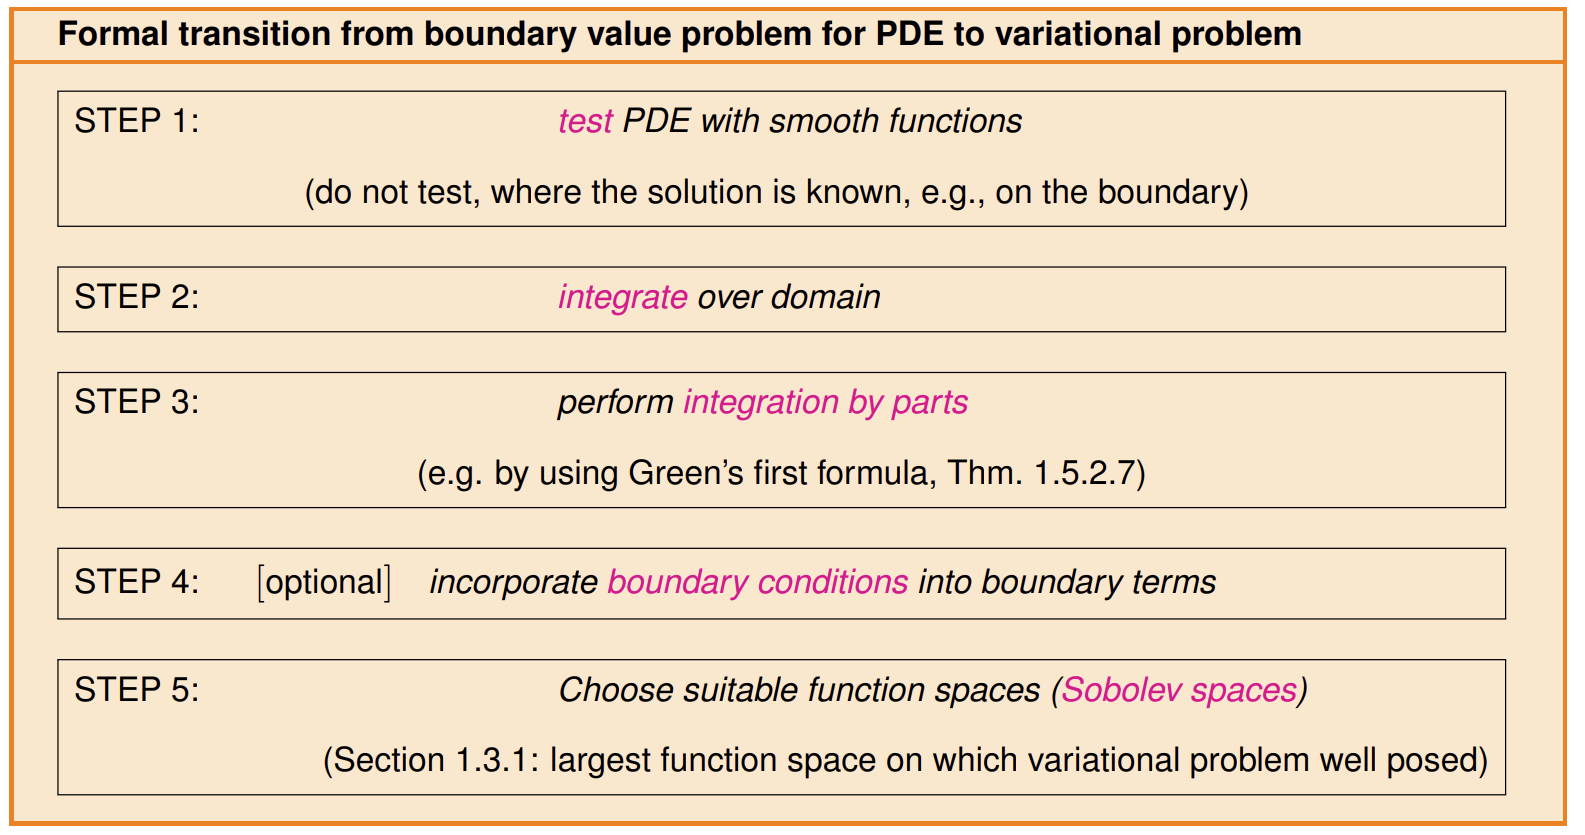
\includegraphics[]{week02/pde_to_lvp_1.png}
\end{figure}


\SubSectionWith{On the continuity of the linear functional}{15min}

TODO: PREPARE EQUATIONS + INTRODUCE EXISTENCE AND UNIQUENESS THM

existence:

energy norm, a bilinear s.p.d
$$||u||_a := (a(u,u))^\frac{1}{2}$$
existence of solution: linear functional has to be bounded wrt to the energy norm $$l(u) \leq C||u||_a$$

Multiplicative Trace Inequality, Pointcarré-Friedrich Inequality, CSI, Triangle Inequality

Show how linear functional of exercise 1.6 is bounded with respect to the energy norm induced by bilinear form a.

\begin{figure}
    \centering
    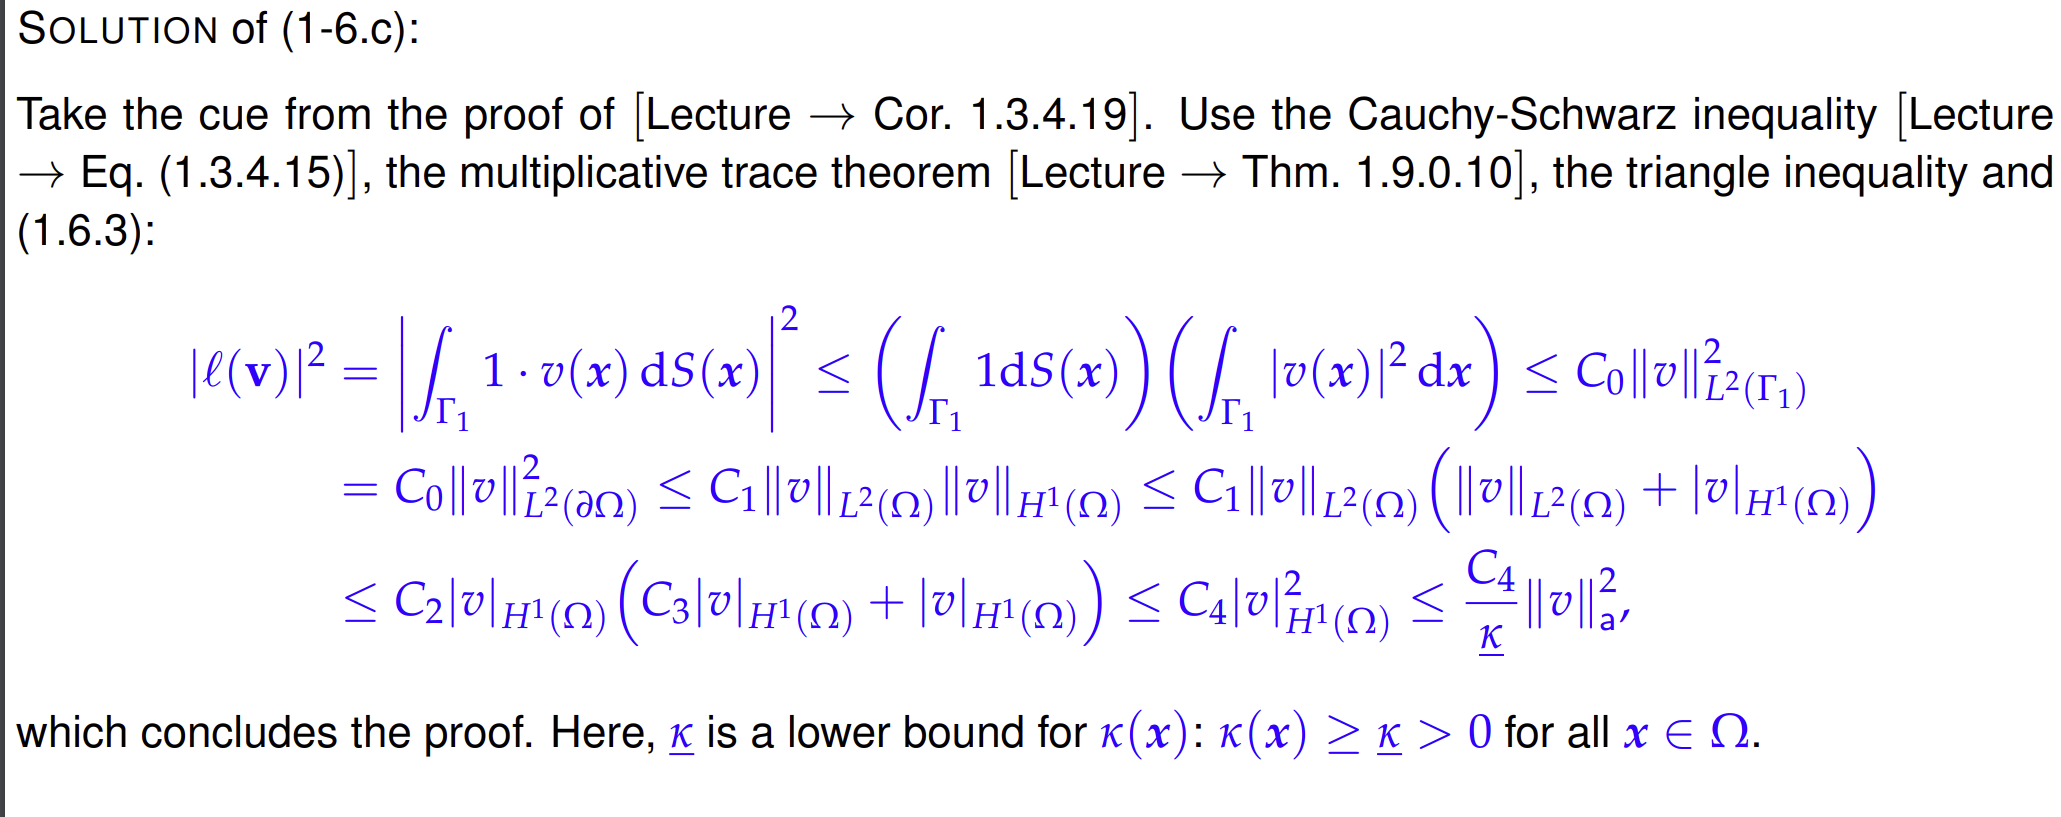
\includegraphics{week02/ex_1_6_c.png}
\end{figure}

\end{document}
